\documentclass{article}
\usepackage{amsmath}
\usepackage{hyperref}
\usepackage{graphicx}
\usepackage{float}
\usepackage[top=2cm]{geometry}

\title{Deep Learning - Homework 1}
\author{99222 - Frederico Silva, 99326 - Sebastião Carvalho}
\date{\today}

\begin{document}

\maketitle

\tableofcontents

\section{Question 1}

Medical image classification with linear classifiers and neural networks.

\subsection{Question 1.1}

\subsubsection{Question 1.1 a)}

\paragraph{Answer} After running the code, the following plot was generated:
\begin{figure}[H]
    \centering
    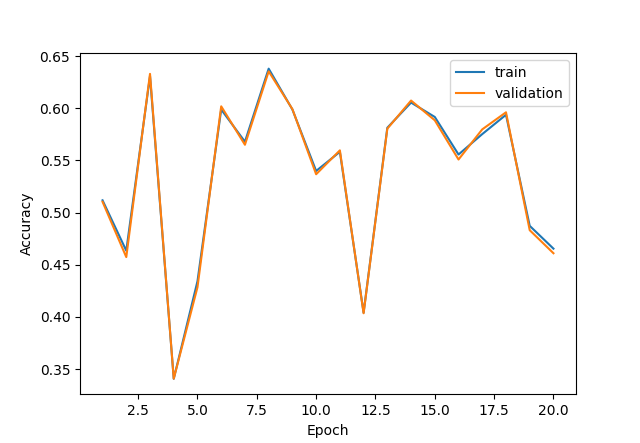
\includegraphics[width=0.8\textwidth]{"plots/1_1_a.png"}
    \caption{Perceptron Training and Validation Accuracy}
    \label{1.1.a Plot}
\end{figure}

The final test accuracy was 0.3422.

\subsubsection{Question 1.1 b)}
\paragraph{Answer} After running the code, the following plots were generated for learning rates $\eta = 0.01$ and $\eta = 0.001$, respectively:
\begin{figure}[H]
    \centering
    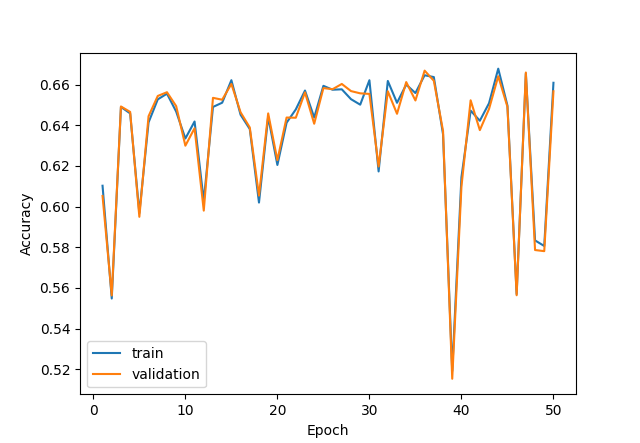
\includegraphics[width=0.8\textwidth]{"plots/1_1_b_001.png"}
    \caption{Logistic Regression Accuracy with Learning Rate $\eta = 0.01$}
    \label{1.1.b 0.01 Plot}
\end{figure}

\begin{figure}[H]
    \centering
    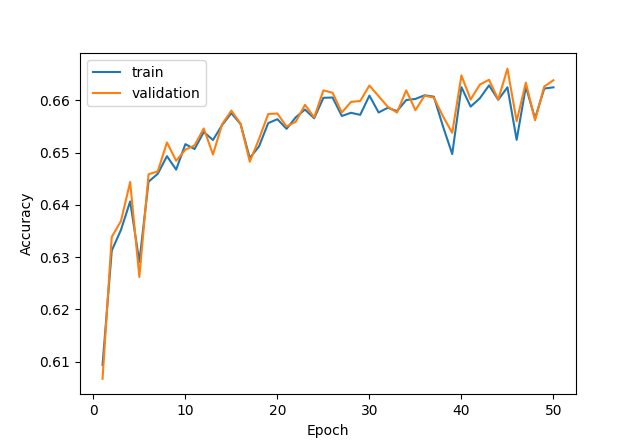
\includegraphics[width=0.8\textwidth]{"plots/1_1_b_0001.png"}
    \caption{Logistic Regression Accuracy with Learning Rate $\eta= 0.001$}
    \label{1.1.b 0.0001 Plot}
\end{figure}

The final test accuracy was 0.5784 and 0.5936 for $\eta = 0.01$ and $\eta = 0.001$ respectively.\\
Comparing both charts, we can see that for $\eta = 0.001$, the accuracy increases more slowly, but it reaches a higher value than for $\eta = 0.01$. 
This is because for $\eta = 0.01$, the algorithm is taking too big steps, and it is not able to converge to a better solution. This can be 
seen in the chart for $\eta = 0.01$, near epoch 40, when the accuracy drops to an all time low.\\
Since the learning rate is too small for $\eta = 0.001$, the algorithm takes longer to reach higher accuracies, but it's also 
less oscillatory, and it is able to converge to a better solution.\\

\subsection{Question 1.2}

\subsubsection{Question 1.2 a)}

\paragraph{Answer}
The answer to this question mainly focus on two topics: how complex the models are, meaning their expressiveness, and how easy they are to train. \\
Regarding the expressiveness, logistic regression is a linear model that learns a single decision boundary to separate classes. 
When using pixel values as features, it treats each pixel independently and cannot capture complex patterns such as shapes or textures 
that might be essential for tasks like image classification.\\ 
On the other hand, a multi-layer perceptron can learn non-linear decision boundaries due to its hidden layers and non-linear activation functions like ReLU. 
Each layer can transform the feature space in a way that makes the data linearly separable by subsequent layers, allowing the MLP to capture 
complex patterns and relationships in the data.\\
When it comes to how easy it is to train this models, logistic regression, with its convex cost function, offers a straightforward training guaranteed 
to reach the global minimum, given enough time and proper learning hyperparameters. 
However, when talking of a multi-layer perceptron, the presence of multiple layers and non-linearities in an MLP makes the optimization landscape non-convex. 
There can be multiple local minima, saddle points, and plateaus. Finding the global minimum is not guaranteed, making the training process, 
most of the times, more complex.\\
In short, the claim is true. A logistic regression model is less expressive than a multi-layer perceptron with ReLU activations because it can only 
represent linear relationships, whereas MLPs can capture non-linearities. Logistic regression models are easier to train because they involve 
convex optimization, unlike the non-convex problem of training MLPs.

\subsubsection{Question 1.2 b)}

\section{Question 2}
Medical image classification with an autodiff toolkit.

\subsection{Question 2.1}

\paragraph{Answer} After running the code, the following plots were generated:

\begin{figure}[H]
    \centering
    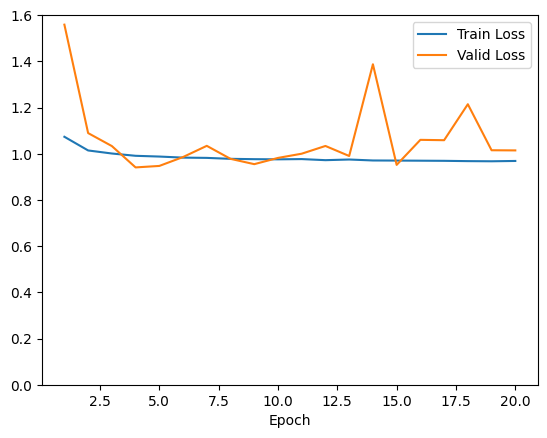
\includegraphics[width=0.8\textwidth]{"plots/logistic_regression-training-loss-batch-16-lr-0.1-epochs-20-l2-0-opt-sgd.png"}
    \caption{Training and validation loss for $\eta = 0.1$}
    \label{2.1 0.1 Loss Plot}
\end{figure}

\begin{figure}[H]
    \centering
    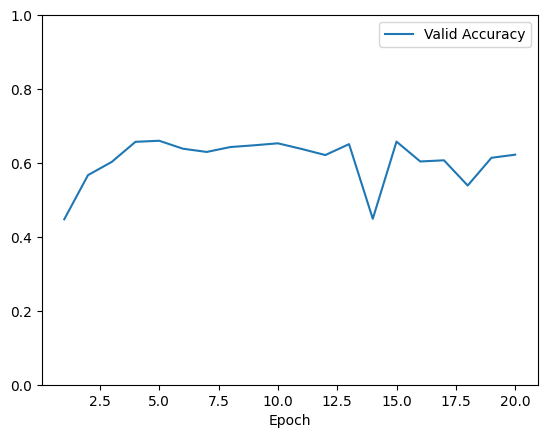
\includegraphics[width=0.8\textwidth]{"plots/logistic_regression-validation-accuracy-batch-16-lr-0.1-epochs-20-l2-0-opt-sgd.png"}
    \caption{Validation accuracy for $\eta = 0.1$}
    \label{2.1 0.1 Acc Plot}
\end{figure}

\begin{figure}[H]
    \centering
    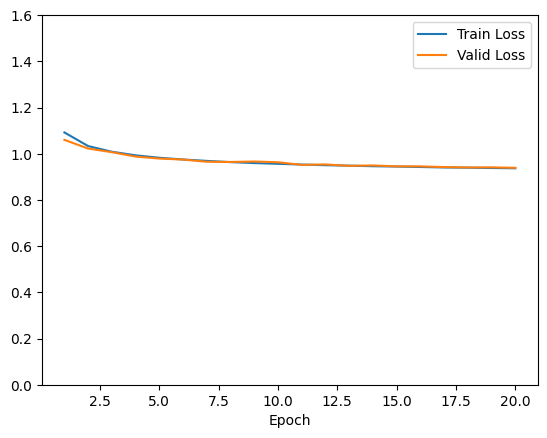
\includegraphics[width=0.8\textwidth]{"plots/logistic_regression-training-loss-batch-16-lr-0.01-epochs-20-l2-0-opt-sgd.png"}
    \caption{Training and validation loss for $\eta = 0.01$}
    \label{2.1 0.01 Loss Plot}
\end{figure}

\begin{figure}[H]
    \centering
    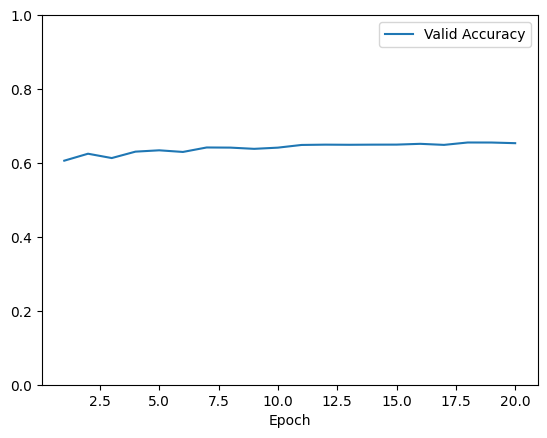
\includegraphics[width=0.8\textwidth]{"plots/logistic_regression-validation-accuracy-batch-16-lr-0.01-epochs-20-l2-0-opt-sgd.png"}
    \caption{Validation accuracy for $\eta = 0.01$}
    \label{2.1 0.01 Acc Plot}
\end{figure}

\begin{figure}[H]
    \centering
    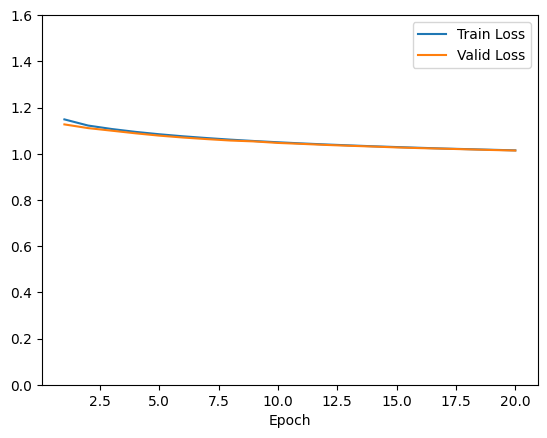
\includegraphics[width=0.8\textwidth]{"plots/logistic_regression-training-loss-batch-16-lr-0.001-epochs-20-l2-0-opt-sgd.png"}
    \caption{Training and validation loss for $\eta = 0.001$}
    \label{2.1 0.001 Loss Plot}
\end{figure}

\begin{figure}[H]
    \centering
    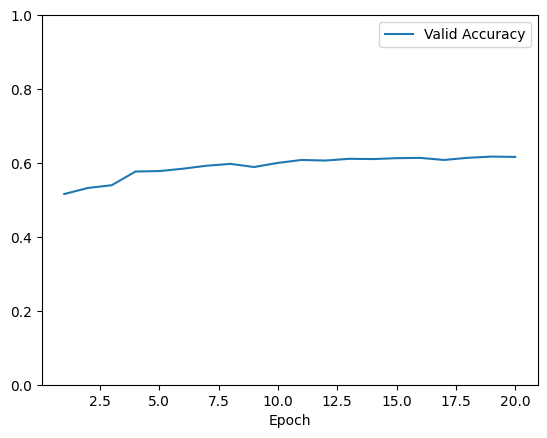
\includegraphics[width=0.8\textwidth]{"plots/logistic_regression-validation-accuracy-batch-16-lr-0.001-epochs-20-l2-0-opt-sgd.png"}
    \caption{Validation accuracy for $\eta = 0.001$}
    \label{2.1 0.001 Acc Plot}
\end{figure}

The test accuracies were 0.5577, 0.6200 and 0.6503 for $\eta = 0.1$, $\eta = 0.01$ and $\eta = 0.001$ respectively.\\
Looking at the plots, we can see that the best configuration, in terms of final valdiation accuracy, was $\eta = 0.01$.\\

\subsection{Question 2.2}

\subsubsection{Question 2.2 a)}
\subsubsection{Question 2.2 b)}
\subsubsection{Question 2.2 c)}

\section{Question 3}

\subsection{Question 3.1}
\subsubsection{Question 3.1 a)}
\paragraph{Answer}

To demonstrate that the specified Boolean function cannot be computed by a single perceptron, let's consider a simple case where \( D = 2 \), \( A = -1 \), and \( B = 1 \). The function \( f \) is defined as:

\[
f(x) = 
\begin{cases} 
1 & \text{if } \sum_{i=1}^{D} x_i \in [-1, 1], \\
-1 & \text{otherwise}
\end{cases}
\]

In this setup:

\begin{itemize}
    \item For \( x = (+1, +1) \), the sum \( \sum x_i = 2 \). Since 2 is not in the range [-1, 1], \( f(x) = -1 \).
    \item For \( x = (-1, -1) \), the sum \( \sum x_i = -2 \). Since -2 is also not in the range [-1, 1], \( f(x) = -1 \).
    \item For \( x = (-1, +1) \) or \( x = (+1, -1) \), the sum \( \sum x_i = 0 \). This falls within the range [-1, 1], so \( f(x) = 1 \) for these inputs.
\end{itemize}

The visual representation of the points can be seen in Figure \ref{3a Plot}. The red points represent the inputs that should be classified as \( +1 \) and the blue points represent the inputs that should be classified as \( -1 \).

The critical point here is that a single perceptron is fundamentally a linear classifier, which means it can only separate data points using a straight line in the feature space. However, in this example, there is no straight line that can separate these points accordingly in a 2D space, to satisfy the function \( f \).

This example thus serves as a counter-example proving that the given function cannot generally be computed with a single perceptron, as it requires a non-linear decision boundary which a single perceptron cannot provide. 

\begin{figure}[H]
    \centering
    \includegraphics[width=0.8\textwidth]{"3a.png"}
    \caption{Classification of points using the function \( f \)}
    \label{3a Plot}
\end{figure}
\subsubsection{Question 3.1 b)}
\subsubsection{Question 3.1 c)}

\end{document}
